%% LyX 2.3.6 created this file.  For more info, see http://www.lyx.org/.
%% Do not edit unless you really know what you are doing.
\documentclass[english,xcolor=svgnames, handout]{beamer}
\usepackage{amsbsy}
\usepackage{amstext}
\usepackage{fontspec}
\setcounter{secnumdepth}{3}
\setcounter{tocdepth}{3}
\usepackage{float}
\usepackage{graphicx}
\ifx\hypersetup\undefined
  \AtBeginDocument{%
    \hypersetup{unicode=true}
  }
\else
  \hypersetup{unicode=true}
\fi

\makeatletter

%%%%%%%%%%%%%%%%%%%%%%%%%%%%%% LyX specific LaTeX commands.
%% Because html converters don't know tabularnewline
\providecommand{\tabularnewline}{\\}

%%%%%%%%%%%%%%%%%%%%%%%%%%%%%% Textclass specific LaTeX commands.
% this default might be overridden by plain title style
\newcommand\makebeamertitle{\frame{\maketitle}}%
% (ERT) argument for the TOC
\AtBeginDocument{%
  \let\origtableofcontents=\tableofcontents
  \def\tableofcontents{\@ifnextchar[{\origtableofcontents}{\gobbletableofcontents}}
  \def\gobbletableofcontents#1{\origtableofcontents}
}

%%%%%%%%%%%%%%%%%%%%%%%%%%%%%% User specified LaTeX commands.

% you can play with different themes and color themes to find your favorite combination.
\mode<presentation> {
  \usetheme{Luebeck}
  \usecolortheme{beaver}
  \beamertemplatenavigationsymbolsempty
}

\usepackage{mathtools}
\usepackage{graphicx} % for including images
\usepackage{pgf} % for logo
\usepackage{colortbl}
\usepackage{booktabs}
\usepackage{emoji}
\usepackage{listings}
\usepackage[many]{tcolorbox}
\usepackage{tabularx}
\usepackage{array}
\tcbuselibrary{skins}
%\usepackage{fdsymbol} % for card symbols


\newcolumntype{Y}{>{\raggedleft\arraybackslash}X}
\tcbset{tab2/.style={enhanced, fontupper=\small,
colback=lightgray!10!white,colframe=cobalt!50!black,colbacktitle=lightsteelblue!40!white,
coltitle=black,center title}}

\newcommand\boldblue[1]{\textcolor{cobalt}{\textbf{#1}}}
\newcommand\boldorange[1]{\textcolor{burntoranger}{\textbf{#1}}}
\def\*#1{\mathbf{#1}}

\date{} % Date, can be changed to a custom date

\titlegraphic{
\vspace{-0.6cm}

\includegraphics[width=1.5cm]{/misc/LogoBlueJustRing.jpg}\break


\tiny
\vspace{1cm}
\href{https://mattiasvillani.com}{
\includegraphics[width=0.33cm]{/misc/web.png} mattiasvillani.com}\hspace*{1cm}~
\href{https://twitter.com/matvil}{
\includegraphics[width=0.3cm]{/misc/twitter.jpg} @matvil}\hspace*{1cm}~
\href{https://fosstodon.org/@matvil}{
\includegraphics[width=0.3cm]{/misc/mastodon.pdf} @matvil}\hspace*{1cm}~
\href{https://github.com/mattiasvillani}{
\includegraphics[width=0.3cm]{/misc/github.png} mattiasvillani}~
}


\definecolor{blue}{RGB}{38, 122, 181}
\definecolor{orange}{RGB}{255, 128, 0}
\definecolor{lorange}{RGB}{255, 178, 102}
\definecolor{llorange}{RGB}{255, 229,204 }
\definecolor{verylightgray}{RGB}{246, 246, 246}
\definecolor{cobalt}{HTML}{0047AB}
\definecolor{lightsteelblue}{HTML}{b0c4de}
\definecolor{lightbluegray}{RGB}{153, 194, 229}

\setbeamertemplate{itemize item}{\color{orange}$\blacksquare$}
\setbeamertemplate{itemize subitem}{\color{orange}$\blacktriangleright$}

\usepackage{tcolorbox}

\newcommand\blfootnote[1]{%
  \begingroup
  \renewcommand\thefootnote{}\footnote{#1}%
  \addtocounter{footnote}{-1}%
  \endgroup
}

\makeatother

\usepackage{polyglossia}
\setdefaultlanguage[variant=american]{english}
\begin{document}
\title[\textcolor{gray}{Bayesian model comparison}]{\textcolor{orange}{Bayesian Learning}}
\subtitle{\textcolor{orange}{Lecture 11 - Bayesian model comparison}}
\author[\textbf{\textcolor{gray}{Mattias Villani}}]{\textbf{Mattias Villani }
\includegraphics[scale=0.02,bb = 0 0 200 100, draft, type=eps]{/home/mv/Dropbox/Teaching/BayesLearning/Misc/Beard Man Emoji.png}
}
\institute[Stockholm University]{Department of Statistics\\
Stockholm University\medskip{}
}
\makebeamertitle
\begin{frame}{\textbf{\textcolor{orange}{Overview}}}

\begin{itemize}
\item \textbf{\textcolor{blue}{Bayesian model comparison}}\textbf{\textcolor{blue}{\small{}\bigskip{}
}}{\small\par}
\item \textbf{\textcolor{blue}{Marginal likelihood}}\textbf{\textcolor{blue}{\small{}\bigskip{}
}}{\small\par}
\end{itemize}
\end{frame}

\begin{frame}{\textbf{\textcolor{orange}{Bayesian model comparison}}}

\begin{itemize}
\item \textbf{\textcolor{blue}{Posterior model probabilities}}
\[
\underset{\text{posterior model prob.}}{\underbrace{\mathrm{Pr}(M_{k}\vert\mathbf{y})}}\propto\underset{\text{marginal likelihood}}{\underbrace{p(\mathbf{y}\vert M_{k})}}\cdot\underset{\text{prior model prob.}}{\underbrace{\mathrm{Pr}(M_{k})}}
\]
\item The \textbf{\textcolor{blue}{marginal likelihood}}\textbf{\textcolor{red}{{}
}}for model $M_{k}$ with parameters $\theta_{k}$
\[
\underbrace{p(\mathbf{y}\vert M_{k})}=\int p(\boldsymbol{y}|\theta_{k},M_{k})p(\theta_{k}|M_{k})d\theta_{k}.
\]
\item $\theta_{k}$ is 'removed' by the averaging wrt prior. \textbf{\textcolor{blue}{Priors
matter!}}\medskip{}
\item The \textbf{\textcolor{blue}{Bayes factor}}
\[
B_{12}(\boldsymbol{y})=\frac{p(\mathbf{y}\vert M_{1})}{p(\mathbf{y}\vert M_{2})}
\]
\end{itemize}
\end{frame}

\begin{frame}{\textbf{\textcolor{orange}{Jeffreys scale of evidence for the Bayes
factor}}}

\begin{itemize}
\item Barely worth mentioning: $1<\mathrm{BF}\leq3$\bigskip{}
\item Positive: $3<\mathrm{BF}\leq20$\bigskip{}
\item Strong: $20<\mathrm{BF}\leq150$\bigskip{}
\item Very strong: $>150$
\end{itemize}
\end{frame}

\begin{frame}{\textbf{\textcolor{orange}{Internet speed data - Bayes factor}}}

\begin{center}
\includegraphics[scale=0.45]{/home/mv/Dropbox/BayesBook/Figs/NormalMargLikeAllKappa0InternetSpeed}
\par\end{center}

\end{frame}

\begin{frame}{\textbf{\textcolor{orange}{Internet speed data - prior predictive
density}}}

\begin{center}
\includegraphics[scale=0.45]{/home/mv/Dropbox/BayesBook/Figs/NormalMargLikeInternetSpeed}
\par\end{center}

\end{frame}

\begin{frame}{\textbf{\textcolor{orange}{Regression example}} }

\end{frame}

\begin{frame}{\textbf{\textcolor{orange}{Laplace approximation}}}

\begin{itemize}
\item Taylor approximation of the log posterior around the posterior mode
$\tilde{\theta}$
\begin{align*}
\ln\left(p(\mathbf{y}|\theta)p(\theta)\right) & \approx\ln p(\mathbf{y}|\tilde{\theta})-\frac{1}{2}J_{\mathbf{y}}(\tilde{\theta})(\theta-\tilde{\theta})^{2}
\end{align*}
so
\begin{align*}
p(\mathbf{y}|\theta)p(\theta) & \approx p(\mathbf{y}|\tilde{\theta})\exp\left[-\frac{1}{2}J_{\mathbf{y}}(\tilde{\theta})(\theta-\tilde{\theta})^{2}\right]p(\hat{\theta})\\
 & =p(\mathbf{y}|\tilde{\theta})p(\tilde{\theta})(2\pi)^{p/2}\left\vert J_{\mathbf{y}}^{-1}(\tilde{\theta})\right\vert ^{1/2}\\
 & \times\underset{\text{multivariate normal density}}{\underbrace{(2\pi)^{-p/2}\left\vert J_{\mathbf{y}}^{-1}(\tilde{\theta})\right\vert ^{-1/2}\exp\left[-\frac{1}{2}J_{\mathbf{y}}(\tilde{\theta})(\theta-\tilde{\theta})^{2}\right]}}
\end{align*}
\item \textbf{\textcolor{blue}{The Laplace approximation}}: 
\[
\ln\hat{p}(\mathbf{y})=\ln p(\mathbf{y}|\tilde{\theta})+\text{ln}p(\tilde{\theta})+\frac{1}{2}\ln\left\vert J_{\mathbf{y}}^{-1}(\tilde{\theta})\right\vert +\frac{p}{2}\ln(2\pi),
\]
where $p$ is the number of unrestricted parameters. 
\end{itemize}
\end{frame}

\begin{frame}{\textbf{\textcolor{orange}{Laplace approximation and BIC}}}

\begin{itemize}
\item \textbf{\textcolor{blue}{The Laplace approximation}}: 
\[
\ln\hat{p}(\mathbf{y})=\ln p(\mathbf{y}|\tilde{\theta})+\text{ln}p(\tilde{\theta})+\frac{1}{2}\ln\left\vert J_{\mathbf{y}}^{-1}(\tilde{\theta})\right\vert +\frac{p}{2}\ln(2\pi)
\]
\medskip{}
\item $\hat{\theta}$ and $J_{\mathbf{y}}(\tilde{\theta})$ can be obtained
with \textbf{\textcolor{blue}{optimization}}/\textbf{\textcolor{blue}{autodiff}}.\bigskip{}
\item The \textbf{\textcolor{blue}{BIC approximation}} 
\[
\ln\hat{p}(\mathbf{y})=\ln p(\mathbf{y}|\hat{\theta})+\ln p(\hat{\theta})-\frac{p}{2}\ln n.
\]
assumes that:
\begin{itemize}
\item $\tilde{\theta}\approx\hat{\theta}$ 
\item $J_{\mathbf{y}}(\tilde{\theta})$ behaves like $n\cdot I_{p}$ in
large samples and 
\item the small term $\frac{p}{2}\ln(2\pi)$ is ignored.
\end{itemize}
\end{itemize}
\end{frame}

\begin{frame}{\textbf{\textcolor{orange}{$\mathrm{Pr}(M_{k}\vert\boldsymbol{y})$
can be overfident - macroeconomics}}\footnote{\href{https://arxiv.org/abs/2003.04026}{Oelrich et al (2020). When are Bayesian model probabilities overconfident?}}}

\begin{table}[H]
\caption{Posterior model probabilities - Smets-Wouters DSGE model}

\centering{}%
\begin{tabular}{ccccccccc}
\hline 
Base & M1 & M2 & M3 & M4 & M5 & M6 & M7 & M8\tabularnewline
0.01 & 0.00 & 0.00 & 0.99 & 0.00 & 0.00 & 0.00 & 0.00 & 0.00\tabularnewline
\hline 
\end{tabular}
\end{table}

\begin{center}
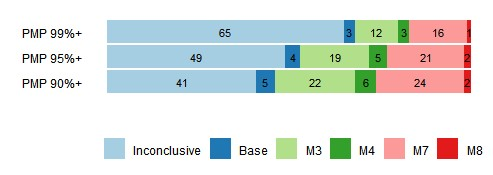
\includegraphics[scale=0.6]{Images/plot_conclusive_evidence}
\par\end{center}

\end{frame}

\begin{frame}{\textbf{\textcolor{orange}{And hey! ... let's be careful out there}}}
¨

\begin{itemize}
\item Be especially \textbf{\textcolor{blue}{careful}} with Bayesian model
comparison when\medskip{}

\begin{itemize}
\item The \textbf{\textcolor{blue}{compared models }}are 

\begin{itemize}
\item very different in structure
\item severly misspecified
\item very complicated (black boxes).\bigskip{}
\end{itemize}
\item The \textbf{\textcolor{blue}{priors}} for the parameters in the models
are 

\begin{itemize}
\item not carefully elicited
\item only weakly informative
\item not matched across models.\bigskip{}
\end{itemize}
\item The \textbf{\textcolor{blue}{data}} 

\begin{itemize}
\item has outliers (in all models)
\item has a multivariate response.
\end{itemize}
\end{itemize}
\end{itemize}
\end{frame}


\end{document}
